\subsection{Алгоритмы получения метеоданных}

Необходимыми данными для вычисления параметров волновой активности являются данные о скорости и направлении ветра.
В разделе~\ref{sec:whether_models} были описаны существующие глобальные модели метеоданных и открытые источники доступа к ним.
Выполненный в нем анализ показал, что наиболее перспективной к использованию моделью является ERA5 с пространственным разрешением в четверть градуса.

Ограничения, вызванные низким пространственным разрешением модели, а также резкие изменения в данных, происходящие при переходе границ между смежными ячейками, в программе решаются взвешенной интерполяцией между ближайшими ячейками модели, что, в свою очередь, требует разумного определения границ для запроса данных.

Границы области запроса определяются относительно охвантывающей геометрии, определяемого положением набора рассматриваемых точек.
После чего, по каждому направлению (широта/долгота) строится равномерная сетка центров с шагом равным разрешению используемой климатической модели.
После этого, в случае необходимости, указывается направления дополнительных рядов ячеек, данные из которых будут участвовать в интерполяции.

Дальнейшие варианты запроса определяются спецификой используемого источника данных.
Так, для случая получения данных из Copernicus Climate Data Store, в программе формируется запрос относительно широты и долготы внешних границ определенной сети, а в случае использования сервиса Open-Meteo -- центров ячеек (рисунок~\ref{pic:NVRSK_weather_grid}).

\begin{figure}
    \begin{center}
	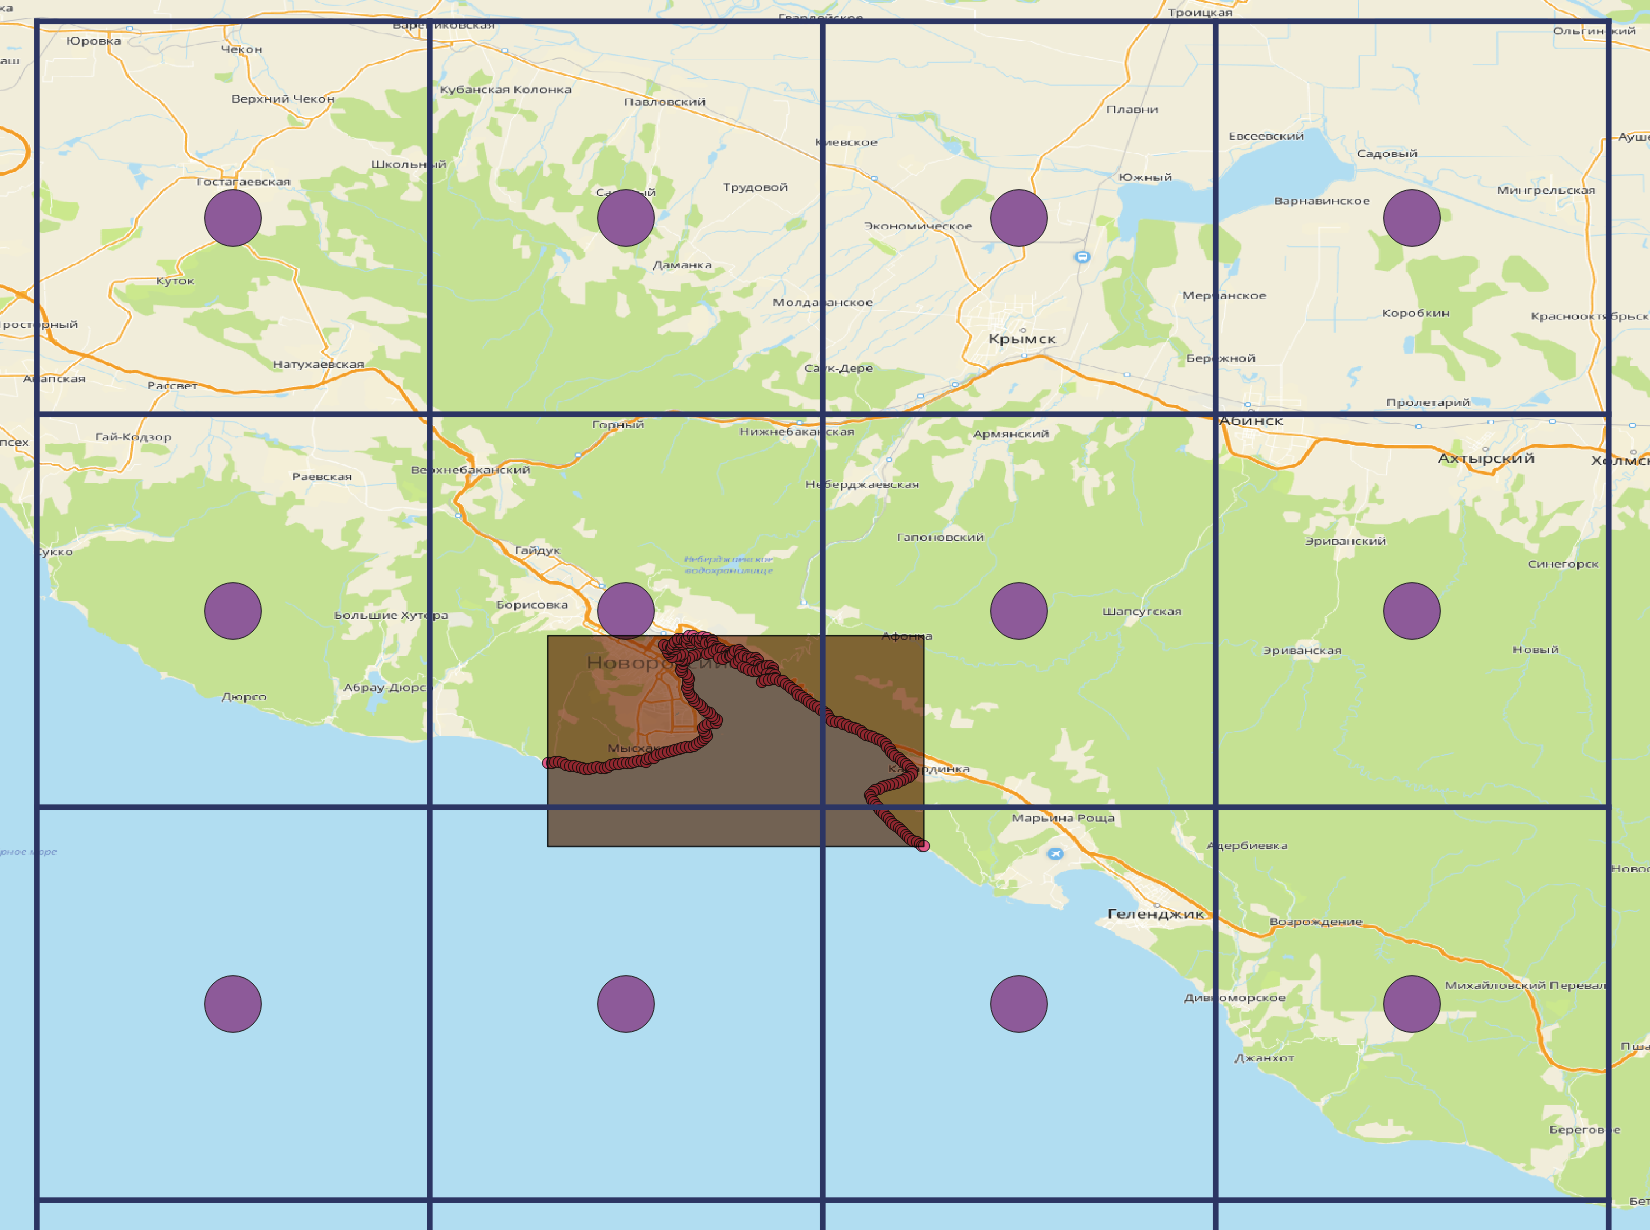
\includegraphics[width=100mm]{fig/part_2/alghoritm/NVRSK_weather_grid.png}
	\caption{-- Распределение данных ERA5 относительно места расчета}
	\label{pic:NVRSK_weather_grid}
    \end{center}
\end{figure}

Описывая текущий опыт получения данных следует отметить, что устойчивый доступ к открытому API Copernicus Climate Data Store, к моменту написания этого текста, установить не удалось.
На текущий момент однозначно установить источник проблем не представляется возможным, но наиболее вероятными причинами могут являться либо неполадки на сервере со стороны источника данных или искусственное ограничение доступа с IP адресов из России.
В то же время функционал формирования и выполнения запроса непосредственно на сайте Climate Data Store продолжает работать и позволяет скачать сырые данные.

С другой стороны источник данных Open-Meteo продолжает работать и позволяет без регистрации выполнить 10 тысяч запросов в сутки.
Опыт работы с этим источником показал, что реальный объем доступных запросов может быть и больше.

В рассматриваемом примере данные о ветре были получены именно из источника Open-Meteo.
Период собранных данных был определен максимально доступным сроком -- начиная от 1 января 1940 года и заканчивая отставанием в пару дней от текущей даты (3 июня 2026 года в работе).

Для исключения лишних запросов при повторных обращениях к серверу в программе был реализован специальный алгоритм кеширования данных.
Для каждой точки сетки и модели создается своя папка внутри которой под каждый запрос формируется пара файлов: \texttt{*.json} с данными и \texttt{*.meta.json} с метаданными запроса. 
Далее набор переменных кодируется в короткий ключ по алгоритму хеширования SHA-256 от отсортированного списка дат.

Чтобы понять, существуют ли данные за запрашиваемый период, происходит проверка равенства полученного и запрашиваемого хеша.
В случае неравенства хешей выполняется детальное сравнение периода запроса и ранее скаченных данных из разности которых формируются подзапросы по отсутствующим временным промежуткам.
После проверки целостности полученных данных хеш от обновленного списка дат обновляется. 

После загрузок всех точек общий кеш еще раз проверяется на полноту по всем датам и формируется выходной \texttt{GeoJSON} по каждой точке сети, в котором все данные за запрашиваемый период сливаются в одну сплошную временную серию.
Таким образом автоматически выполняется условие согласованности порядка данных во всех ячейках модели, позволяющее в гарантировано интерполировать данные для каждой точки в любой день за рассматриваемый период от одних и тех же ячеек сетки метеоданных.

После формирования полного набора метеоданных их ассоциация с конкретной анализируемой точкой производится по двум стратегиям:
\begin{itemize}
    \item по попаданию в ячейку;
    \item методом обратно взвешенного расстояния (IDW).
\end{itemize}

В случае использования первой стратегии каждая береговая точка полностью наследует ряд данных ближайшей погодной точки.
В то время как IDW интерполяция позволяет получить взвешенное значение относительно соседних ячеек метеоданных.

В случае использования IDW стратегии координаты точек переводятся в метрическую CRS и для каждой точки ищутся $k$ ближайших узлов (в пределах $1 \le k \le N$, где $N$ количество ячеек сети метеоданных).
После чего считаются веса:
\begin{equation}
    w_i = \frac{1}{\max(d_i, \varepsilon)^p},\quad p=\text{idw\_power},\ \varepsilon\approx10^{-9}.
\end{equation}

Рассчитанные веса нормируются так, чтобы $\sum_i w_i = 1$.
Для каждой береговой точки и каждого дня скорости ветра берутся как поэлементная взвешенная сумма по $k$ соседним узлам:
\begin{equation}
    v = \sum_i w_i v_i.
\end{equation}

Азимуты направления ветра интерполируются через векторизацию путем вычисления проекций на координатные оси.
Фактически сначала интерполируются значения синуса и косинуса каждого азимута в точке, после чего по формуле~\eqref{eq:azimuth_calc} вычисляется усредненное направление ветра.
Необходимость такого подхода вызвана цикличностью угла и позволяет избежать ошибок, возникающих при усреднении значений в близи перехода между северным направением $360°$ и $0°$.

В результате работы алгоритма интерполяции каждая точка получает собственные значения параметров ветра, позволяя отчасти скомпенсировать низкое пространственное разрешение метео модели.
Пример розы ветров, полученной для первой точки анализируемого участка берега представлен на рисунке~\ref{pic:NVRSK_wind_rose}, из которого видно доминирующее направление северо-восточного ветра, что согласуется с региональным именным ветром -- Новороссийской борой (сильный порывистым северо-восточныо/восточным ветром, дующим с Кавказских гор к Цемесской бухте).

\begin{figure}
    \begin{center}
	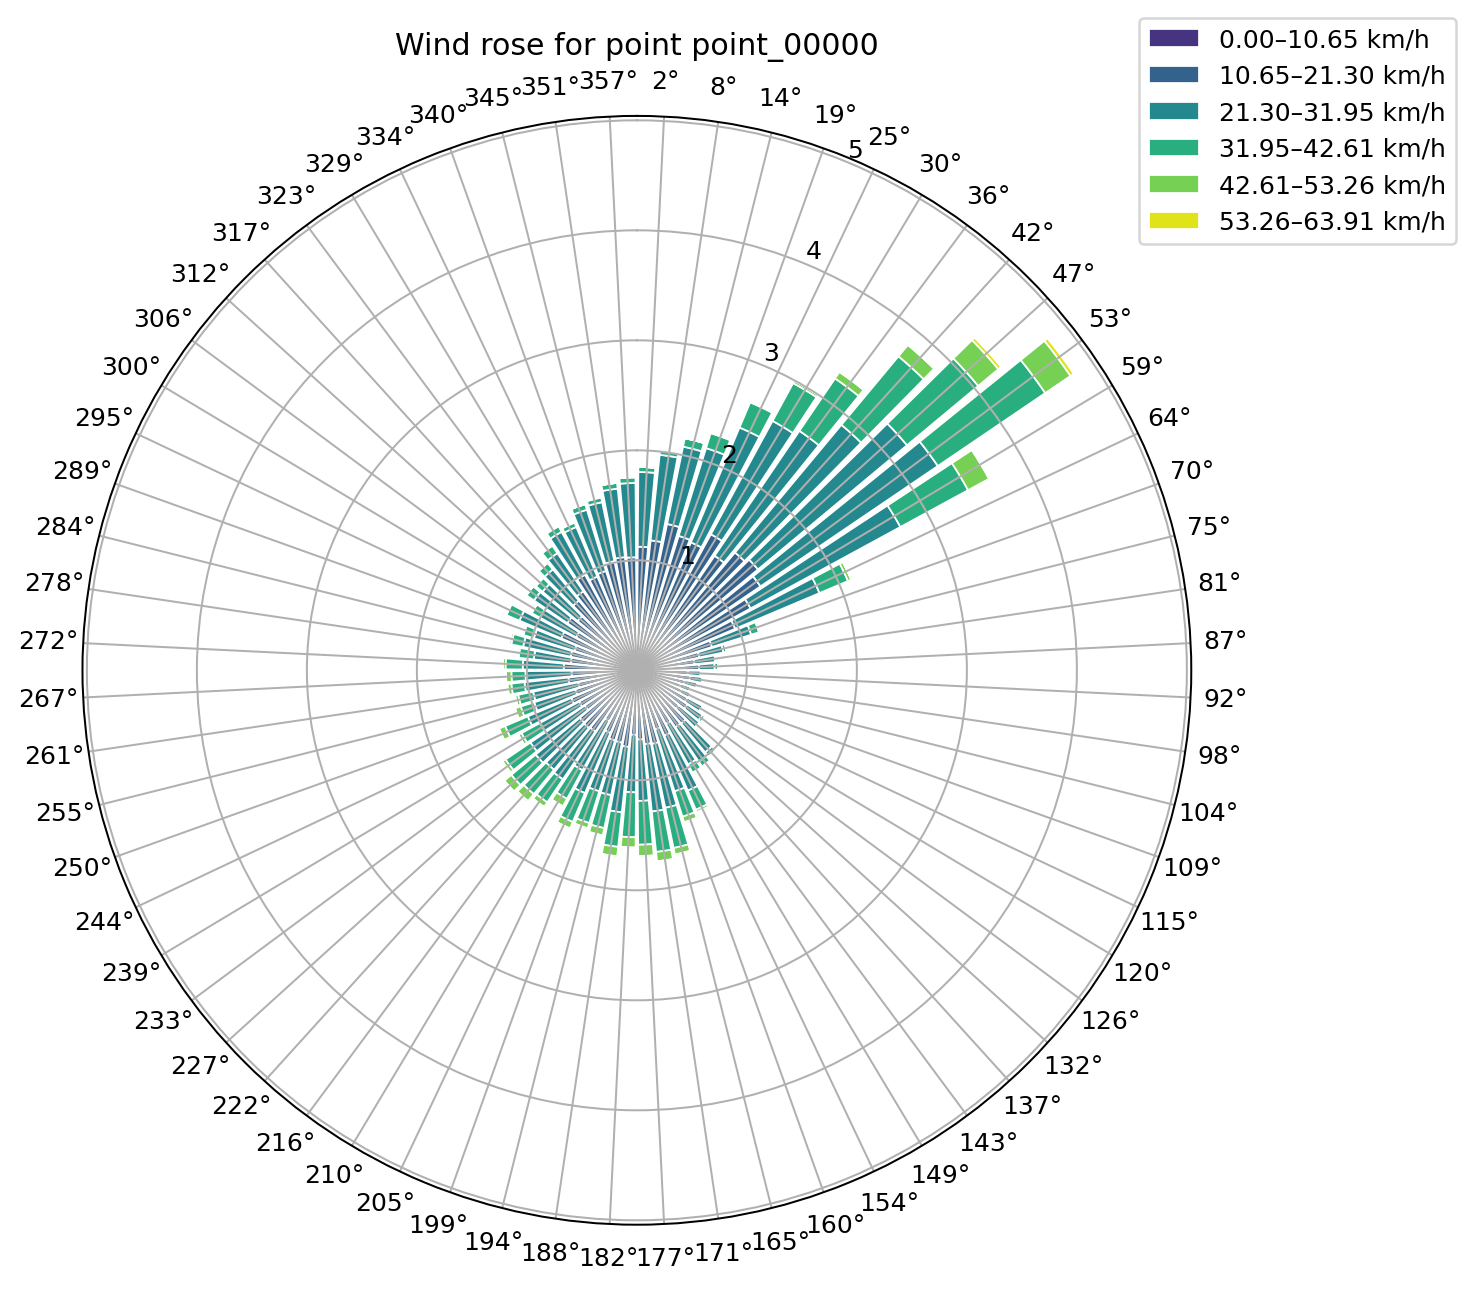
\includegraphics[width=100mm]{fig/part_2/alghoritm/point_00000_wind_rose.png}
	\caption{-- Пример расчитанной розы ветров для первой точки за период с 1 января 1940~г.}
	\label{pic:NVRSK_wind_rose}
    \end{center}
\end{figure}
